\documentclass{article}
\usepackage{tikz}
\usetikzlibrary{shapes, arrows, chains}
\tikzstyle{line} = [draw, -latex']
\begin{document}
	
\title{ExaGEP Plan of Work}

\author{G.~A.}

\maketitle

\section{Representation of Circuits}

\begin{figure}[h]\centering{%
	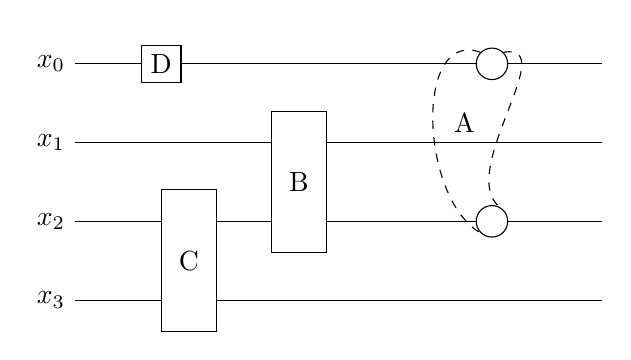
\begin{tikzpicture}
		\def\yl{-1}
		\def\xl{7}
		\node (x0) at (0,0) {$x_0$};
		\node (x1) at (0, \yl) {$x_1$};
		\node (x2) at (0, 2*\yl) {$x_2$};
		\node (x3) at (0, 3*\yl) {$x_3$};
		\coordinate (l0) at (\xl, 0);
		\coordinate (l1) at (\xl, \yl);
		\coordinate (l2) at (\xl, 2*\yl);
		\coordinate (l3) at (\xl, 3*\yl);
		\draw (x0) -- (l0);
		\draw (x1) -- (l1);
		\draw (x2) -- (l2);
		\draw (x3) -- (l3);
		\node[rectangle,draw=black,fill=white] at (0.2*\xl, 0) {D};
		\draw[fill=white] (0.4*\xl, 0.6*\yl) -- (0.5*\xl, 0.6*\yl) -- (0.5*\xl, 2.4*\yl) -- (0.4*\xl, 2.4*\yl) -- cycle;
		\node at (0.45*\xl, 1.5*\yl) {B};
		\draw[fill=white] (0.2*\xl, 1.6*\yl) -- (0.3*\xl, 1.6*\yl) -- (0.3*\xl, 3.4*\yl) -- (0.2*\xl, 3.4*\yl) -- cycle;
		\node at (0.25*\xl, 2.5*\yl) {C};
		\node[circle, draw=black, minimum size=0.4cm, fill=white] (A0) at (0.8*\xl, 0) {};
		\node[circle, draw=black, minimum size=0.4cm, fill=white] (A1) at (0.8*\xl, 2*\yl) {};
		\draw[dashed] (A0.north west) to[out=160, in=150] (A1.south west);
		\draw[dashed] (A0.north east) to[out=10, in=150] (A1.north east);
		\node at (0.75*\xl, 0.75*\yl) {A};
	\end{tikzpicture}}
	\caption{\label{fig:circuit}
		An example of a 4-bit quantum circuit with gates A, B, C, and D in order
		to explain the circuit encoding in genetic expression programming.}
\end{figure}
\begin{figure}[h]\centering{%
	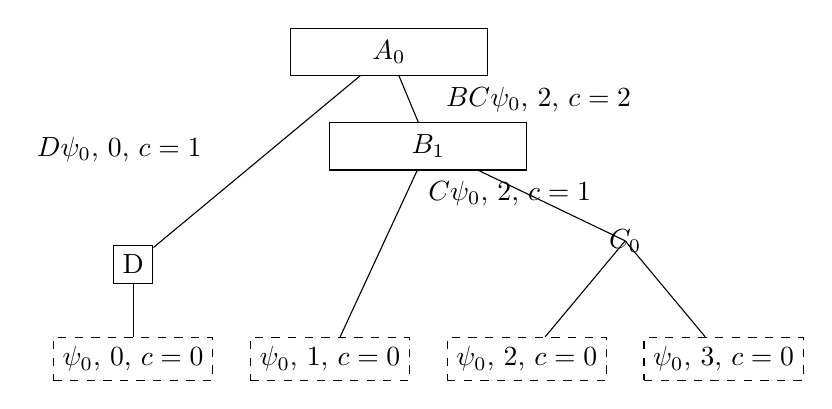
\begin{tikzpicture}
		\def\yn{1.2}
		\def\xn{2.5}
		\node[rectangle, dashed, draw=black] (x0) at (0, 0) {$\psi_0$, 0, $c=0$};
		\node[rectangle, dashed, draw=black] (x1) at (\xn, 0) {$\psi_0$, 1, $c=0$};
		\node[rectangle, dashed, draw=black] (x2) at (2*\xn, 0) {$\psi_0$, 2, $c=0$};
		\node[rectangle, dashed, draw=black] (x3) at (3*\xn, 0) {$\psi_0$, 3, $c=0$};
		\node[rectangle,draw=black,fill=white] (D) at (0, \yn) {D};
		
		\coordinate (C) at (2.5*\xn, 1.25*\yn);	
		\coordinate (B) at (1.5*\xn, 2.25*\yn);
		\coordinate(A) at (1.3*\xn, 3.25*\yn);
		\draw (x0) -- (D);
		\draw (x2) -- (C);
		\draw (x3) -- (C);
		\draw (x1) -- (B);
		%\draw (C) -- (B);
		\path [line] (C) -- node [text width=2.5cm,midway] {$C\psi_0$, 2, $c=1$} (B);		
		%\draw (D) -- (A);
		\path [line] (D) -- node [text width=2.5cm,midway, left=1em] {$D\psi_0$, 0, $c=1$} (A);
		\path [line] (B) -- node [text width=2.5cm,midway, right=1em] {$BC\psi_0$, 2, $c=2$} (A);
		%\draw (B) -- (A);
		
		draw[fill=white] (2*\xn, \yn) -- (3*\xn, \yn) -- (3*\xn, 1.5*\yn) -- (2*\xn, 1.5*\yn) -- cycle;
		\node at (C) {$C_0$};
		\draw[fill=white] (\xn, 2*\yn) -- (2*\xn, 2*\yn) -- (2*\xn, 2.5*\yn) -- (\xn, 2.5*\yn) -- cycle;
		\node at (B) {$B_1$};
		\draw[fill=white] (0.8*\xn, 3*\yn) -- (1.8*\xn, 3*\yn) -- (1.8*\xn, 3.5*\yn) -- (0.8*\xn, 3.5*\yn) -- cycle;
		\node at (A) {$A_0$};
		

		
	\end{tikzpicture}}
\end{figure}

The 4-bit quantum circuit in Fig.~\ref{fig:circuit} will be represented
by the following four genes A$_0$ D$x_0$  B$_1x_1$ C$_0x_2x_3$;
 B$_0x_1$ C$_0x_2x_3$; A$_1$B$_1x_1$C$_0x_2 x_3$; and C$_1x_2x_3$.
Here, A, B, C, and D are gates, the input is to the left, and the output to the right.
Gates A, B, and C take two inputs and produce two outputs. Gate D takes one input and produces one output.

To understand the first gene, consider that it is the first (upper) output of applying
the quantum circuit to the ket $|x_0, x_1, x_2, x_3\rangle$. Therefore, we need
to apply the first output of gate A, indicated by A$_0$ to two inputs, because
gate A takes two inputs. The first (upper) input is the result of applying the D gate
to $x_0$ so we have the first part as A$_0$ D$x_0\ldots$. The second (lower) input to gate
A is the second output of B or B$_1$. Now B has two inputs, one is $x_1$ and the other is
the first output of gate C, which we denote by C$_0$. Combining it all we have so far
A$_0$ D$x_0$ B$_1x_1$C$_0\ldots$. Finally, gate C takes two inputs which are $x_2$ and $x_3$,
yielding the first output or first gene as A$_0$ D$x_0$ B$_1x_1$C$_0x_2x_3$.

\section{Optimization Procedure}
Given a state $|\psi^{\textrm{known}}\rangle$, we want to find a quantum
circuit $\mathcal{C}_{\textrm{unknown}}$ that generates it for an initial state $|\psi_0\rangle$,
that is, that satisfies 
\begin{equation}
	|\psi^{\textrm{known}}\rangle=\mathcal{C}_{\textrm{unknown}}|\psi_0\rangle.
\end{equation}
The genetic expression programming procedure to find such a circuit is as follows.

\begin{enumerate}
	\item Start with an original population of $M=100$ circuits generated randomly.
	\item Start with a pure state ket of length $N$: $|\psi_0\rangle\equiv|x_0, x_1, \ldots, x_{N-1}\rangle$.
	\item By genetic expression programming mutations and combinations of the original 
	population created in step 1, generate $M'=200$ new circuits
	$\{\mathcal{C}(\varphi)\}_{0\le j<M}$. These circuits may depend on
	$K$ continuous variables
	$\varphi\equiv\{\varphi_k\}_{0\le k<K}$. To understand why this is so, consider that the rotation gate
	may depend on the angle of rotation, and, in general, gates may depend on arbitrary parameters that
	we collectively call $\varphi$.
	\item For every circuit $j$, define the $\varphi-$dependent ket $\psi_j(\varphi)\equiv\mathcal{C}_j(\varphi)|\psi_0\rangle$.
	\item For every circuit $j$, define the pre-fitness $P_j$ function by
	\begin{equation}
		P_j(\varphi) \equiv |\langle \psi^{\textrm{known}} | \psi_j(\varphi)\rangle|^2
	\end{equation}
	and find the $\varphi$ where the maximum occurs; let's call it $\varphi_{\textrm{max}}$.
	\item For every circuit $j$, calculate its fitness $F_j \equiv P_j(\varphi_{\textrm{max}})$.
	\item Eliminate the $M'-M=100$ circuits with less fitness and keep the others.
	\item Go to step 3. 
\end{enumerate}
\end{document}

